\documentclass{article}

%%%%%%%%%%%%%%%%%%%%%%%%%%%%%%%%%%%%%%%%%%%%%%%%%%%%%%%%%%%%%%%%%%%%%%%%%%%%%%%%%%%%%%%%%%%%%%%%%%%%%%%%%%%
% 欢迎使用长沙理工大学本科生毕业设计LaTeX样张。
% 作者:陈翊 2023/4/23
% !!! 本模板按照长沙理工大学官网提供的word版样张制作 !!!

% 本样张旨在帮助同学们更方便地使用LaTeX撰写毕业设计,节省繁琐的格式调整时间,更专注于论文的内容撰写。

% 使用本样张,您可以轻松实现以下功能:
% - 自动编号的章节、图表、公式
% - 自动排版参考文献
% - 美观的论文格式和排版效果
% - 方便的分章编写

% 此外,我们还为您提供以下LaTeX写作的小技巧:

% 在正文中引用参考文献,可使用“\cite{引用的文献编号}”命令,如“\cite{Lamport1994}”
% 分章编写可将每个章节单独存为一个.tex文件,再通过“\input{文件名}”命令引入主文件中
% 插入图片的命令为“\includegraphics{图片文件名}”,可设置图片大小、位置等属性
% 插入表格的命令为“\begin{table}...\end{table}”,可设置表格标题、对齐方式等属性
% 希望这些小技巧能够帮助您更好地使用LaTeX,撰写出优秀的毕业设计。

% 如果您希望学习更多LateX技巧以下是几个 LaTeX 教程网站:

% Overleaf 文档:https://www.overleaf.com/learn/latex/Main_Page
% LaTeX 教程 - LaTeX123:http://www.latex123.com/
% LaTeX 入门 - 莫烦 Python:https://morvanzhou.github.io/tutorials/others/latex/
% LaTeX Tutorial - Tutorialspoint:https://www.tutorialspoint.com/latex/index.htm
% LaTeX Notes - Mathematics Department, University of Utah:http://www.math.utah.edu/~beebe/LaTeX/Notes/LaTeX.html
% 这些网站都提供了各种程度的 LaTeX 教程和资料,包括基本语法、排版技巧、数学公式、表格、图形、参考文献等方面的内容。您可以根据自己的需要选择相应的教程网站。
%%%%%%%%%%%%%%%%%%%%%%%%%%%%%%%%%%%%%%%%%%%%%%%%%%%%%%%%%%%%%%%%%%%%%%%%%%%%%%%%%%%%%%%%%%%%%%%%%%%%%%%%%%%

% 配置与格式信息
\usepackage{fancyhdr}
\usepackage{lipsum}
\usepackage{graphicx}
\usepackage[UTF8]{ctex}
\usepackage{amsmath}
\usepackage{lastpage}
\usepackage[top=2.5cm, bottom=2cm, left=3cm, right=2cm]{geometry} % 页边距设定
\usepackage{float}
\usepackage{times} 
\usepackage{mathptmx}
\usepackage{fontspec}
\usepackage[numbers, square, sort&compress]{natbib} % 引入natbib宏包



\renewcommand{\labelenumi}{(\arabic{enumi})} % 将enumerate计数器设置为(1)、(2)、(3)...
\setmainfont{Times New Roman}[BoldFont=Times New Roman Bold]   % 设置英文默认字体
\setcitestyle{super} % 设置引用标注的样式为上标

% ==================================== 全局变量设置 ==================================== 
\newcommand{\thistitle}{一些约束体系量子哈密顿中算符次序问题}     % 设置文章题目
\newcommand{\sanhaolineskip}{\vspace*{16pt}} 
\date{}
% ====================================================================================


% ==================================== 字体字号设置 ==================================== 
\setCJKmainfont{Noto Serif CJK SC} % 指定一个默认字体
\setCJKfamilyfont{hei}{Noto Sans CJK SC} % 定义黑体字体
\setCJKfamilyfont{song}{Noto Serif CJK SC} % 定义宋体字体
\newcommand{\hei}{\CJKfamily{hei}} % 创建一个新的命令 \hei
\newcommand{\song}{\CJKfamily{song}} % 创建一个新的命令 \song


\newcommand{\yihao}{\fontsize{26pt}{36pt}\selectfont}          % 一号, 1.4 倍行距
\newcommand{\erhao}{\fontsize{22pt}{28pt}\selectfont}          % 二号, 1.25倍行距
\newcommand{\xiaoer}{\fontsize{18pt}{18pt}\selectfont}         % 小二, 单倍行距
\newcommand{\sanhao}{\fontsize{16pt}{24pt}\selectfont}         % 三号, 1.5倍行距
\newcommand{\xiaosan}{\fontsize{15pt}{22pt}\selectfont}        % 小三, 1.5倍行距
\newcommand{\sihao}{\fontsize{14pt}{21pt}\selectfont}          % 四号, 1.5 倍行距
\newcommand{\banxiaosi}{\fontsize{13pt}{19.5pt}\selectfont}    % 半小四, 1.5倍行距
\newcommand{\xiaosi}{\fontsize{12pt}{18pt}\selectfont}         % 小四, 1.5倍行距
\newcommand{\dawuhao}{\fontsize{11pt}{11pt}\selectfont}        % 大五号, 单倍行距
\newcommand{\wuhao}{\fontsize{10.5pt}{15.75pt}\selectfont}     % 五号, 单倍行距
\newcommand{\xiaowu}{\fontsize{9pt}{9pt}\selectfont} % 小五号, 单倍行距
% ==================================================================================


% ==================================== 目录格式设定 ====================================
\usepackage{titletoc}
% \contentsmargin{2.5em} % 设置目录和页码之间的距离
\renewcommand{\contentsname}{\heiti\sanhao 目\quad\ 录}
\dottedcontents{section}[1.5em]{\xiaosi\hei}{1.5em}{1pc} % 小节目录的格式
\dottedcontents{subsection}[3.5em]{\xiaosi\song}{2em}{1pc} % 子节目录的格式
\dottedcontents{subsubsection}[5.5em]{\xiaosi\song}{2.5em}{1pc} % 子节目录的格式
% ====================================================================================


% ==================================== 定义标题格式 ==================================== 
\usepackage{titlesec}
\titlespacing{\section}{0pt}{0pt}{\baselineskip}
\titleformat{\section}{\centering\hei\xiaosan}{\thesection}{1em}{}
\titleformat{\subsection}{\hei\sihao}{\thesubsection}{1em}{}
\titleformat{\subsubsection}{\hei\xiaosi}{\quad\quad\thesubsubsection}{1em}{}
% ===================================================================================


% ==================================== 图序和图题设置 ==================================
\usepackage{caption}
\usepackage{chngcntr}
\DeclareCaptionFont{wuhaosong}{\fontsize{10.5pt}{15.75pt}\selectfont \song} % 设置字体为宋体,五号
\captionsetup[figure]{font=wuhaosong, labelfont=wuhaosong, labelsep=quad} % 设置图题字体为宋体,五号,标号和图名之间的距离为一个空格
\counterwithin{figure}{section} % 将图号计数器设置为随着每个章节编号重新计数
\DeclareCaptionLabelFormat{myfiglabel}{\thesection.#2} % 定义新的图标签格式
% ==================================================================================


% ==================================== 设置表格标题格式 ================================
\DeclareCaptionFont{wuhaosongcu}{\fontsize{10.5pt}{15.75pt}\selectfont \song\bfseries} % 设置字体为宋体,五号
\captionsetup[table]{
    labelsep=quad, % 标签与标题内容之间的距离
    font={ wuhaosongcu }, % 字体样式:小五、加粗、黑体
    skip=1pt, % 标题与表格之间的距离
    format=plain, % 标题的格式:不加冒号
    singlelinecheck=false, % 标题超过一行时居左
    justification=centering, % 标题居中
}
\renewcommand{\thetable}{\arabic{section}-\arabic{table}}   % 设置表格题目为“章节号-章节内序号”
% ==================================================================================


% ==================================== 公式格式设置 ==================================== 
% 公式序号设置为(所在章节号-章节内编号)
\numberwithin{equation}{section}
\renewcommand{\theequation}{\thesection-\arabic{equation}}
\usepackage[italic]{mathastext} % 将数学字体设置为默认字体

% ==================================================================================


% ==================================== 代码格式设定 ====================================
\usepackage{xcolor}
\usepackage{listings}
% 用来设置附录中代码的样式

\lstset{
    basicstyle          =   \sffamily,          % 基本代码风格
    keywordstyle        =   \bfseries,          % 关键字风格
    commentstyle        =   \rmfamily\itshape,  % 注释的风格,斜体
    stringstyle         =   \ttfamily,  % 字符串风格
    flexiblecolumns,                % 别问为什么,加上这个
    numbers             =   left,   % 行号的位置在左边
    showspaces          =   false,  % 是否显示空格,显示了有点乱,所以不现实了
    numberstyle         =   \zihao{-5}\ttfamily,    % 行号的样式,小五号,tt等宽字体
    showstringspaces    =   false,
    captionpos          =   t,      % 这段代码的名字所呈现的位置,t指的是top上面
    frame               =   lrtb,   % 显示边框
}

\lstdefinestyle{Python}{
    language        =   Python, % 语言选Python
    basicstyle      =   \zihao{-5}\ttfamily,
    numberstyle     =   \zihao{-5}\ttfamily,
    keywordstyle    =   \color{blue},
    keywordstyle    =   [2] \color{teal},
    stringstyle     =   \color{magenta},
    commentstyle    =   \color{red}\ttfamily,
    breaklines      =   true,   % 自动换行,建议不要写太长的行
    columns         =   fixed,  % 如果不加这一句,字间距就不固定,很丑,必须加
    basewidth       =   0.5em,
}
% ==================================================================================

\begin{document}
    
    % 页眉页脚设置
    \pagestyle{fancy}
    \fancyhf{}
    \lhead{
\includegraphics[width=5cm]{./img/csust.png}}
    \rhead{\hei\xiaowu\thistitle}
    \renewcommand{\headrulewidth}{0.4pt}

    \thispagestyle{fancy} % 保留页眉和页脚

    % ============================= 中文摘要 ==========================
    \begin{center}
        \vspace*{16pt} % 空一行
        \hei\sanhao{\thistitle}
    \end{center}
    \vspace*{14pt} % 空一行
    \begin{center} 
        \hei\xiaosan{摘要}
        \vspace*{16pt} % 空一行
    \end{center}
    

\song\xiaosi 长沙理工大学(Changsha University of Science \& Technology),简称“CSUST”,位于湖南省长沙市,是国家交通运输部和湖南省人民政府共建高校 ,属于湖南省“国内一流大学建设高校”(A类),入选“中西部高校基础能力建设工程”、教育部“卓越工程师教育培养计划”、教育部“大学生创新性实验计划”,是中国电力高校联盟、绿色交通联盟、中俄交通大学联盟成员之一,是全国毕业生就业典型经验高校,全国深化创新创业教育改革示范高校。

长沙理工大学由原长沙交通学院、长沙电力学院于2003年合并组建。原长沙交通学院的前身是交通部1956年创办的长沙航务工程学校,原长沙电力学院的前身是电力工业部1956年创办的长沙水力发电学校。创办于1956年的湖南省水利水电学校和创办于1958年的湖南省轻工业学校(后更名为湖南轻工业高等专科学校)相继于2001年和2002年并入原长沙电力学院。

截至2022年11月,学校有金盆岭、云塘两个校区,占地面积2980亩,校舍总建筑面积140余万平方米,图书馆纸本藏书360万册;有22个教学学院,1个独立学院、1个继续教育学院,85个本科专业;拥有博士后科研流动站5个,一级学科博士学位授权点8个,二级学科博士学位授权点42个,博士专业学位授权点1个,一级学科硕士学位授权点29个,二级学科硕士学位授权点134个,硕士专业学位授权点18个,5个学科进入ESI全球排名前1\%;有专任教师近2100人,在校生45000余人(含城南学院7000余人),其中硕士、博士研究生8500余人。

\vspace{\baselineskip}
\noindent \sihao\hei 关键词: \song\xiaosi 长沙理工大学;本科毕业论文;模板


    \clearpage

    % ============================= 英文摘要 ==========================
    \begin{center}
        \vspace*{16pt} % 空一行
         \textbf{\sanhao THE OPERATOR ORDERING PROBLEM IN QUANTUM HAMITONIAN FOR SOME CONSTRAINT SYSTEMS}
    \end{center}
    \vspace*{14pt} % 空一行
    \begin{center}
        \textbf{\xiaosan ABSTRACT}
        \vspace*{16pt} % 空一行
    \end{center}
    \xiaosi 
\quad\quad \lipsum[1-2]


    
\vspace{\baselineskip}
\noindent \sihao\textbf{ Key words:} \xiaosi Lorem; ipsum; Foo; Bar
    \clearpage
    % ================================================================
   

    % ============================= 目录 ============================
    \vspace*{16pt} % 空一行
    \tableofcontents
    % ================================================================


    % ==========================  正文页眉页码设置  ===================
    
    % 页码设置
    \clearpage % 确保在新页面开始
    \thispagestyle{fancy}
    \pagenumbering{arabic} % 设置页码格式为阿拉伯数字
    \setcounter{page}{1} % 设置页码起始值为3

    % 页眉页脚设置
    \pagestyle{fancy}
    \fancyhf{}
    \lhead{
\includegraphics[width=5cm]{./img/csust.png}}
    \rhead{\thistitle}
    % \cfoot{\thepage}
    \cfoot{第 \thepage\ 页 \hspace{0.5em}\ 共 \pageref{LastPage}\ 页}
    \renewcommand{\headrulewidth}{0.4pt}
    % ================================================================
    

    % ==========================  正文开始  ==========================
    \clearpage
    \sanhaolineskip
    \section{绪论}
        \subsection{课题背景及目的}
            \xiaosi
Lorem ipsum \citep{agrawal2011challenges} dolor sit amet, consectetuer adipiscing elit. Ut purus elit, vestibulum ut,
placerat ac, adipiscing vitae, felis. Curabitur dictum gravida mauris. Nam arcu libero, nonummy
eget, consectetuer id, vulputate a, magna. Donec vehicula augue eu neque. Pellentesque habitant
morbi tristique senectus et netus et malesuada fames ac turpis egestas. Mauris ut leo. Cras
viverra metus rhoncus sem. Nulla et lectus vestibulum urna fringilla ultrices. Phasellus eu tellus
sit amet tortor gravida placerat. Integer sapien est, iaculis in, pretium quis, viverra ac, nunc.
Praesent eget sem vel leo ultrices bibendum. Aenean faucibus. Morbi dolor nulla, malesuada eu,
pulvinar at, mollis ac, nulla. Curabitur auctor semper nulla. Donec varius orci eget risus. Duis
nibh mi, congue eu, accumsan eleifend, sagittis quis, diam\cite{wu2013data}. Duis eget orci sit amet orci dignissim
rutrum.\cite{zhang2016}

\begin{figure}[H]
    \centering
    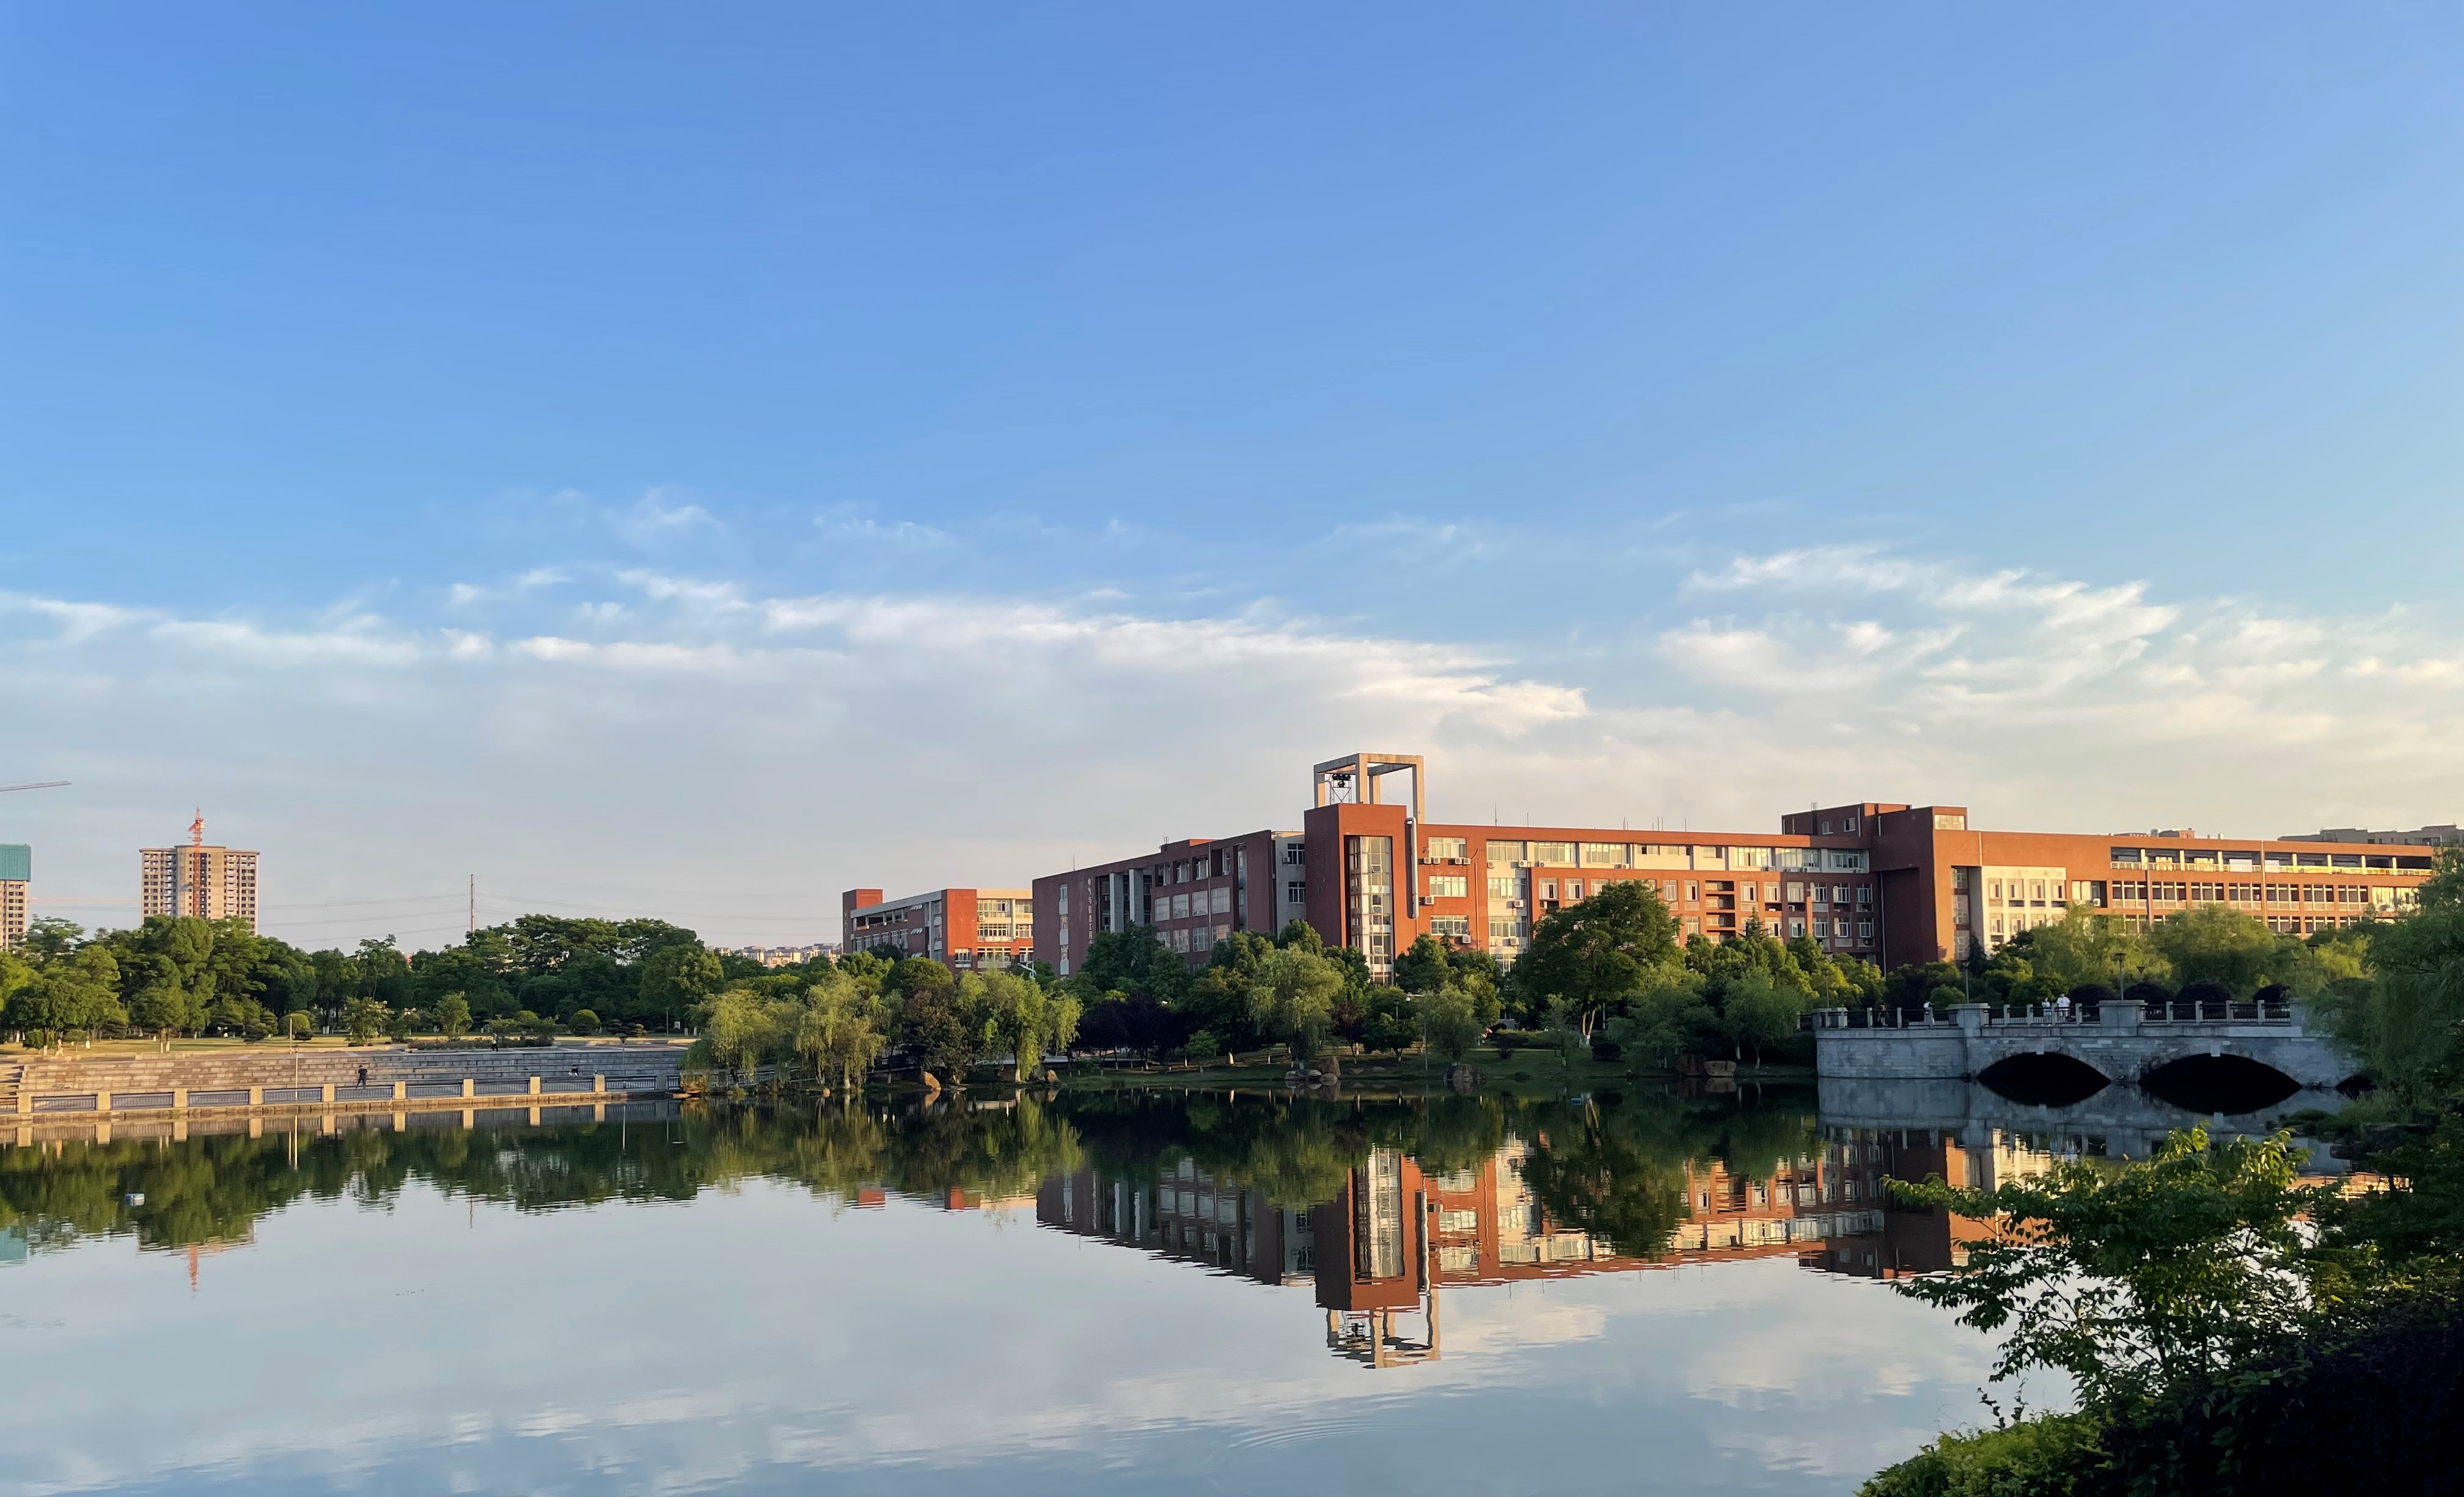
\includegraphics[width=0.8\linewidth]{img/fig1.jpg}
    \caption{一张示例图片}
    \label{fig:figure1}
\end{figure}

\lipsum[1-2]


        \subsection{国内外研究状况}
            \subsubsection{国外研究现状}
                \xiaosi

\lipsum[1-2]

\begin{equation}
     \sum_{i=\left\lceil\frac{m}{2}\right\rceil}^{m}\left(\begin{array}{c}
     m \\
     i
     \end{array}\right) p^{i}(1-p)^{m-i}=\sum_{i=0}^{\left\lfloor\frac{m}{2}\right\rfloor}\left(\begin{array}{c}
     m \\
     i
     \end{array}\right)(1-p)^{i} p^{m-i}
\end{equation}

\lipsum[1]

\begin{equation}
    \begin{aligned}
        \operatorname{Pr}\left\{o_{k}^{*} \!\succeq \!r\! \succeq \!o_{c k}^{*} \mid x, m\right\}\!=\!1 & \!-\!\sum_{i=\left\lceil\frac{m}{2}\right\rceil}^{m}\!\left(\!\begin{array}{c}
        m \\
        i
        \end{array}\right) p^{i}(1\!-\!p)^{m\!-\!i} \\
        & \!-\!\sum_{i=\left\lceil\frac{m+1}{2}\right\rceil}^{m}\!\left(\!\begin{array}{c}
        m \\
        i
        \end{array}\right) q^{m\!-\!i}(1\!-\!q)^{i}
    \end{aligned}
\end{equation}
            \subsubsection{国内研究现状}
                \xiaosi 

\lipsum[1]

\begin{enumerate}
    \item 分项1
    \item 分项2
    \item 分项3
\end{enumerate}

\lipsum[1]
        \subsection{本章小结}
            \xiaosi 

\lipsum[1]

\begin{figure}[H]
    \centering
    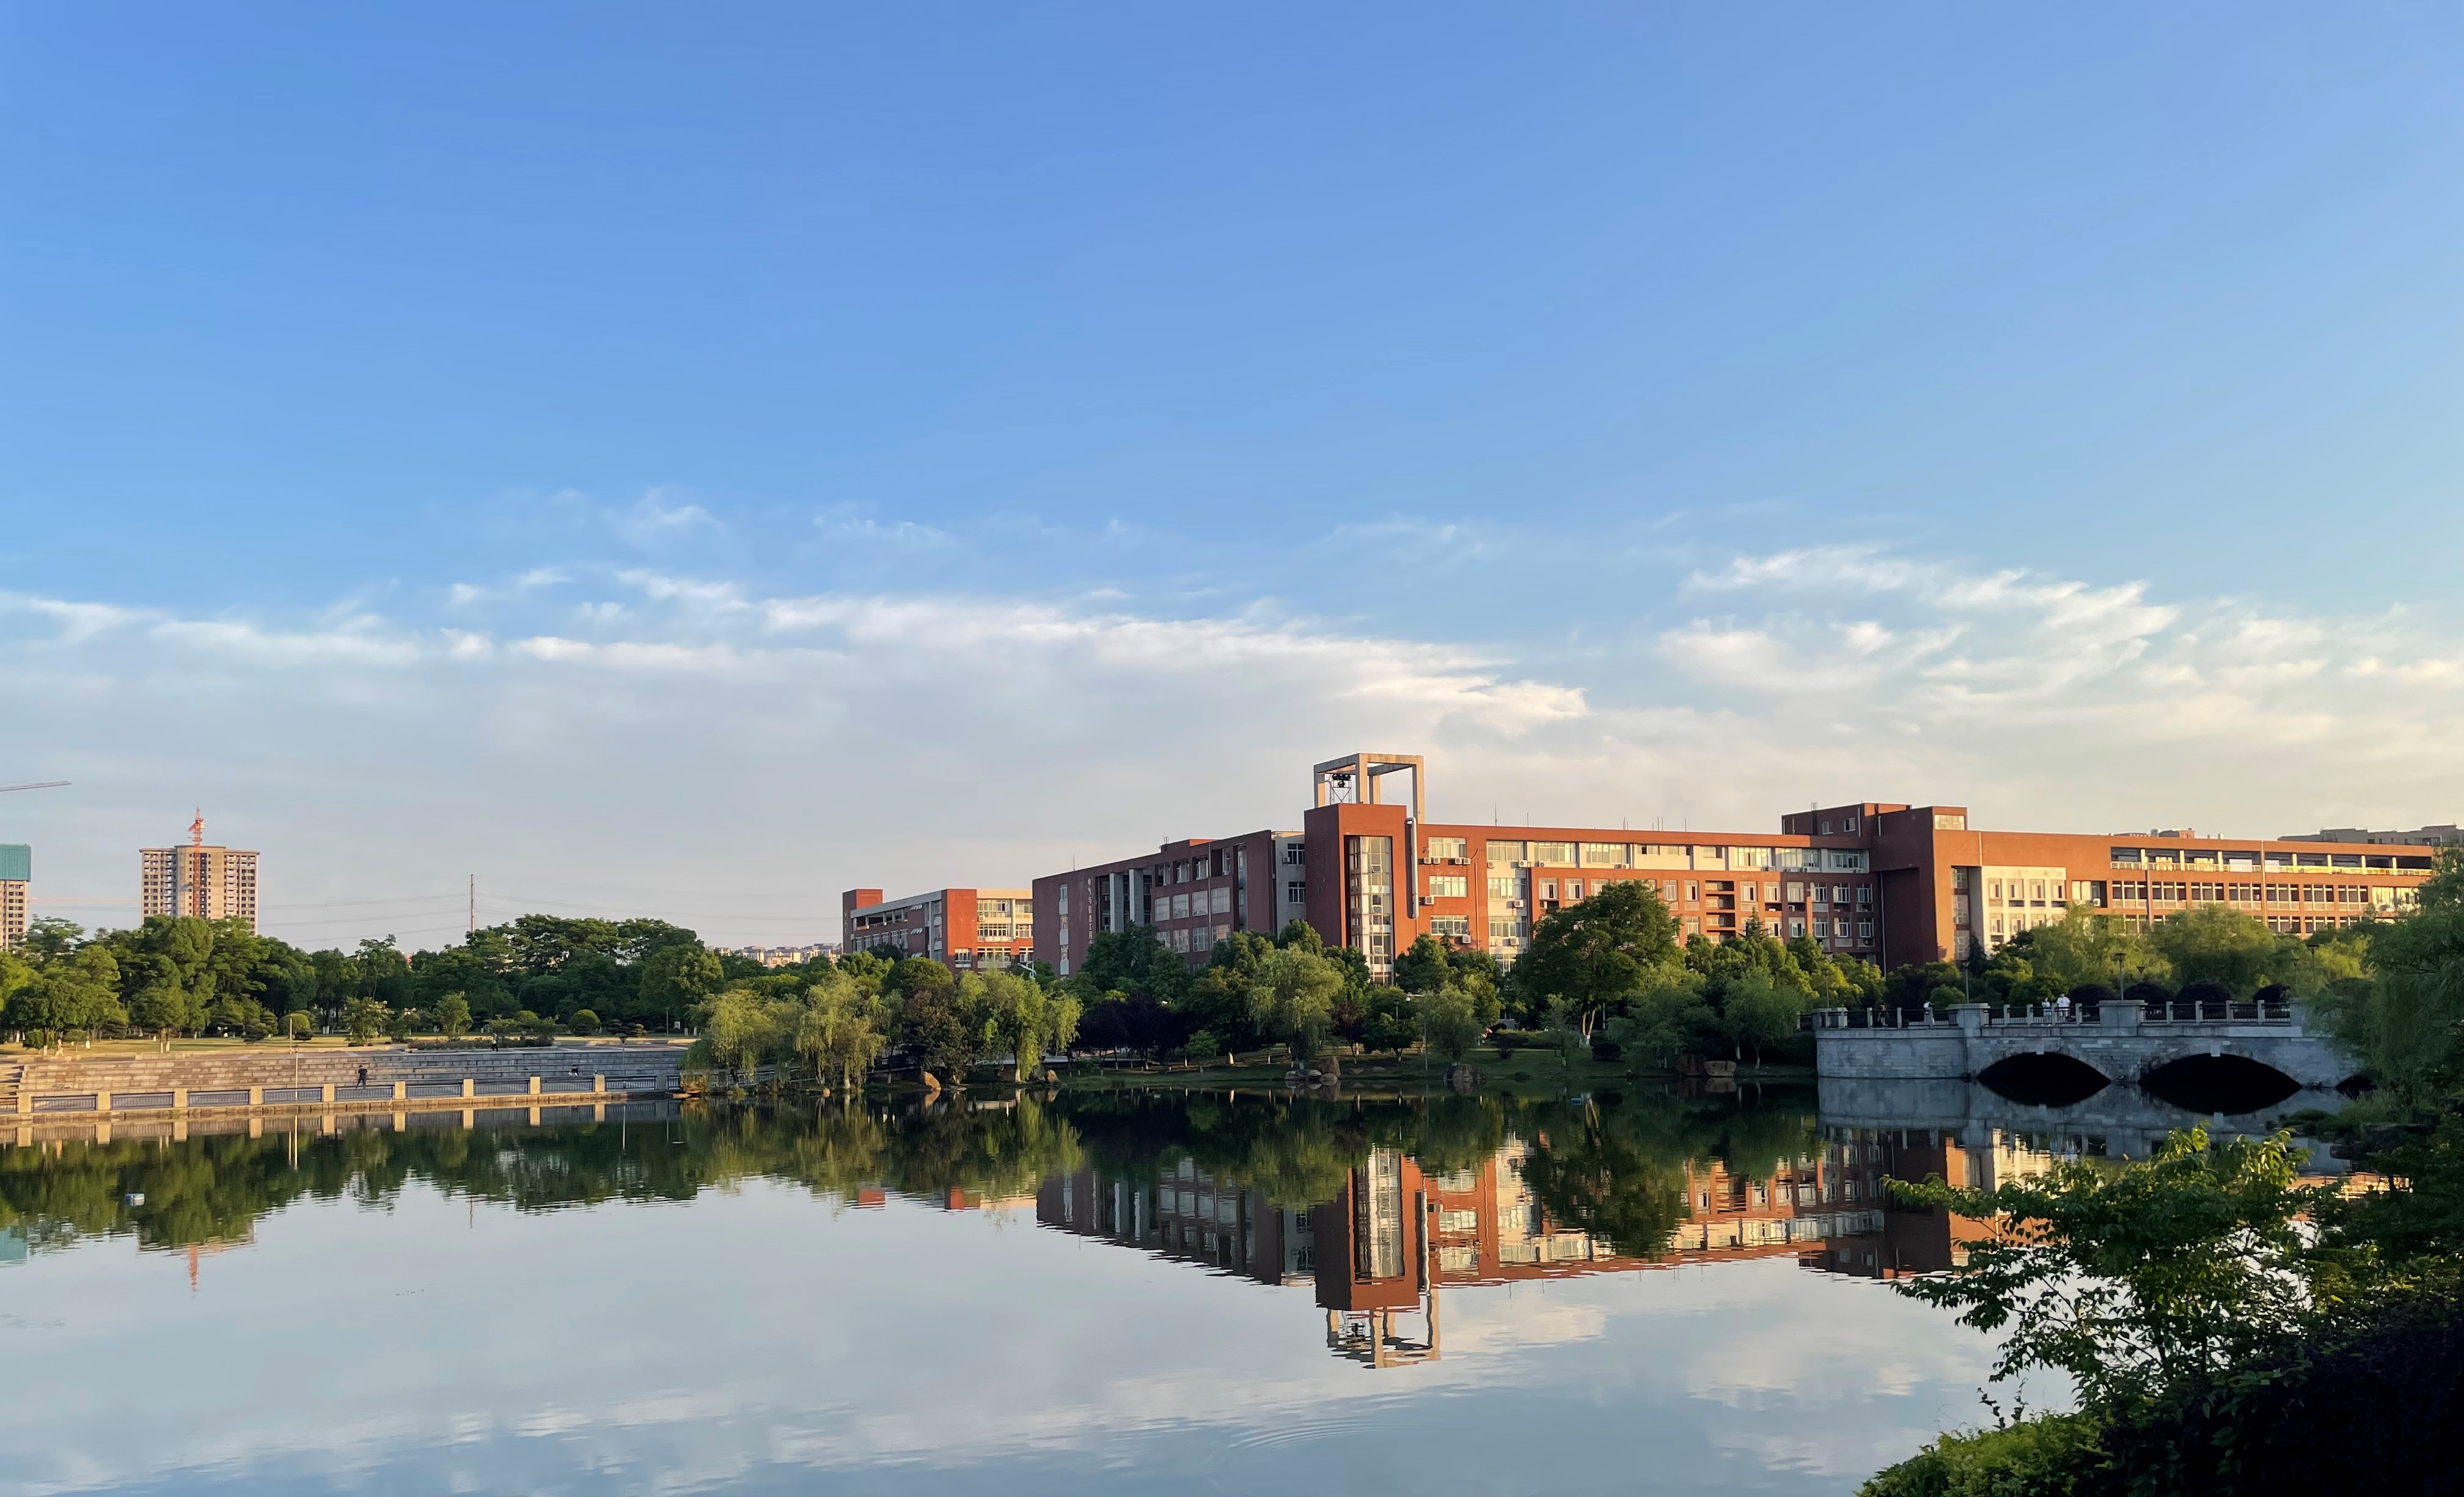
\includegraphics[width=0.8\linewidth]{img/fig1.jpg}
    \caption{注意图例图题}
    \label{fig:figure2}
\end{figure}

\lipsum[1-2]

    \clearpage
    \sanhaolineskip
    \section{相关技术介绍}
        \subsection{技术一}
            \xiaosi 
\lipsum[1]

\wuhao
\begin{table}[H]
  \centering
  \caption{表格标题}
  \label{tab:my-table}
  \begin{tabular}{|c|c|c|}
    \hline
    字段名 & 字段类型 & 是否为空 \\
    \hline
    id & int & NOT NULL \\
    \hline
    name & varchar(20) & NOT NULL \\
    \hline
    age & int & NULL \\
    \hline
  \end{tabular}
\end{table}







\lipsum[1]
        \subsection{技术二}
            \xiaosi

\lipsum[1-2]



\lipsum[1-2]

\begin{figure}[H]
    \centering
    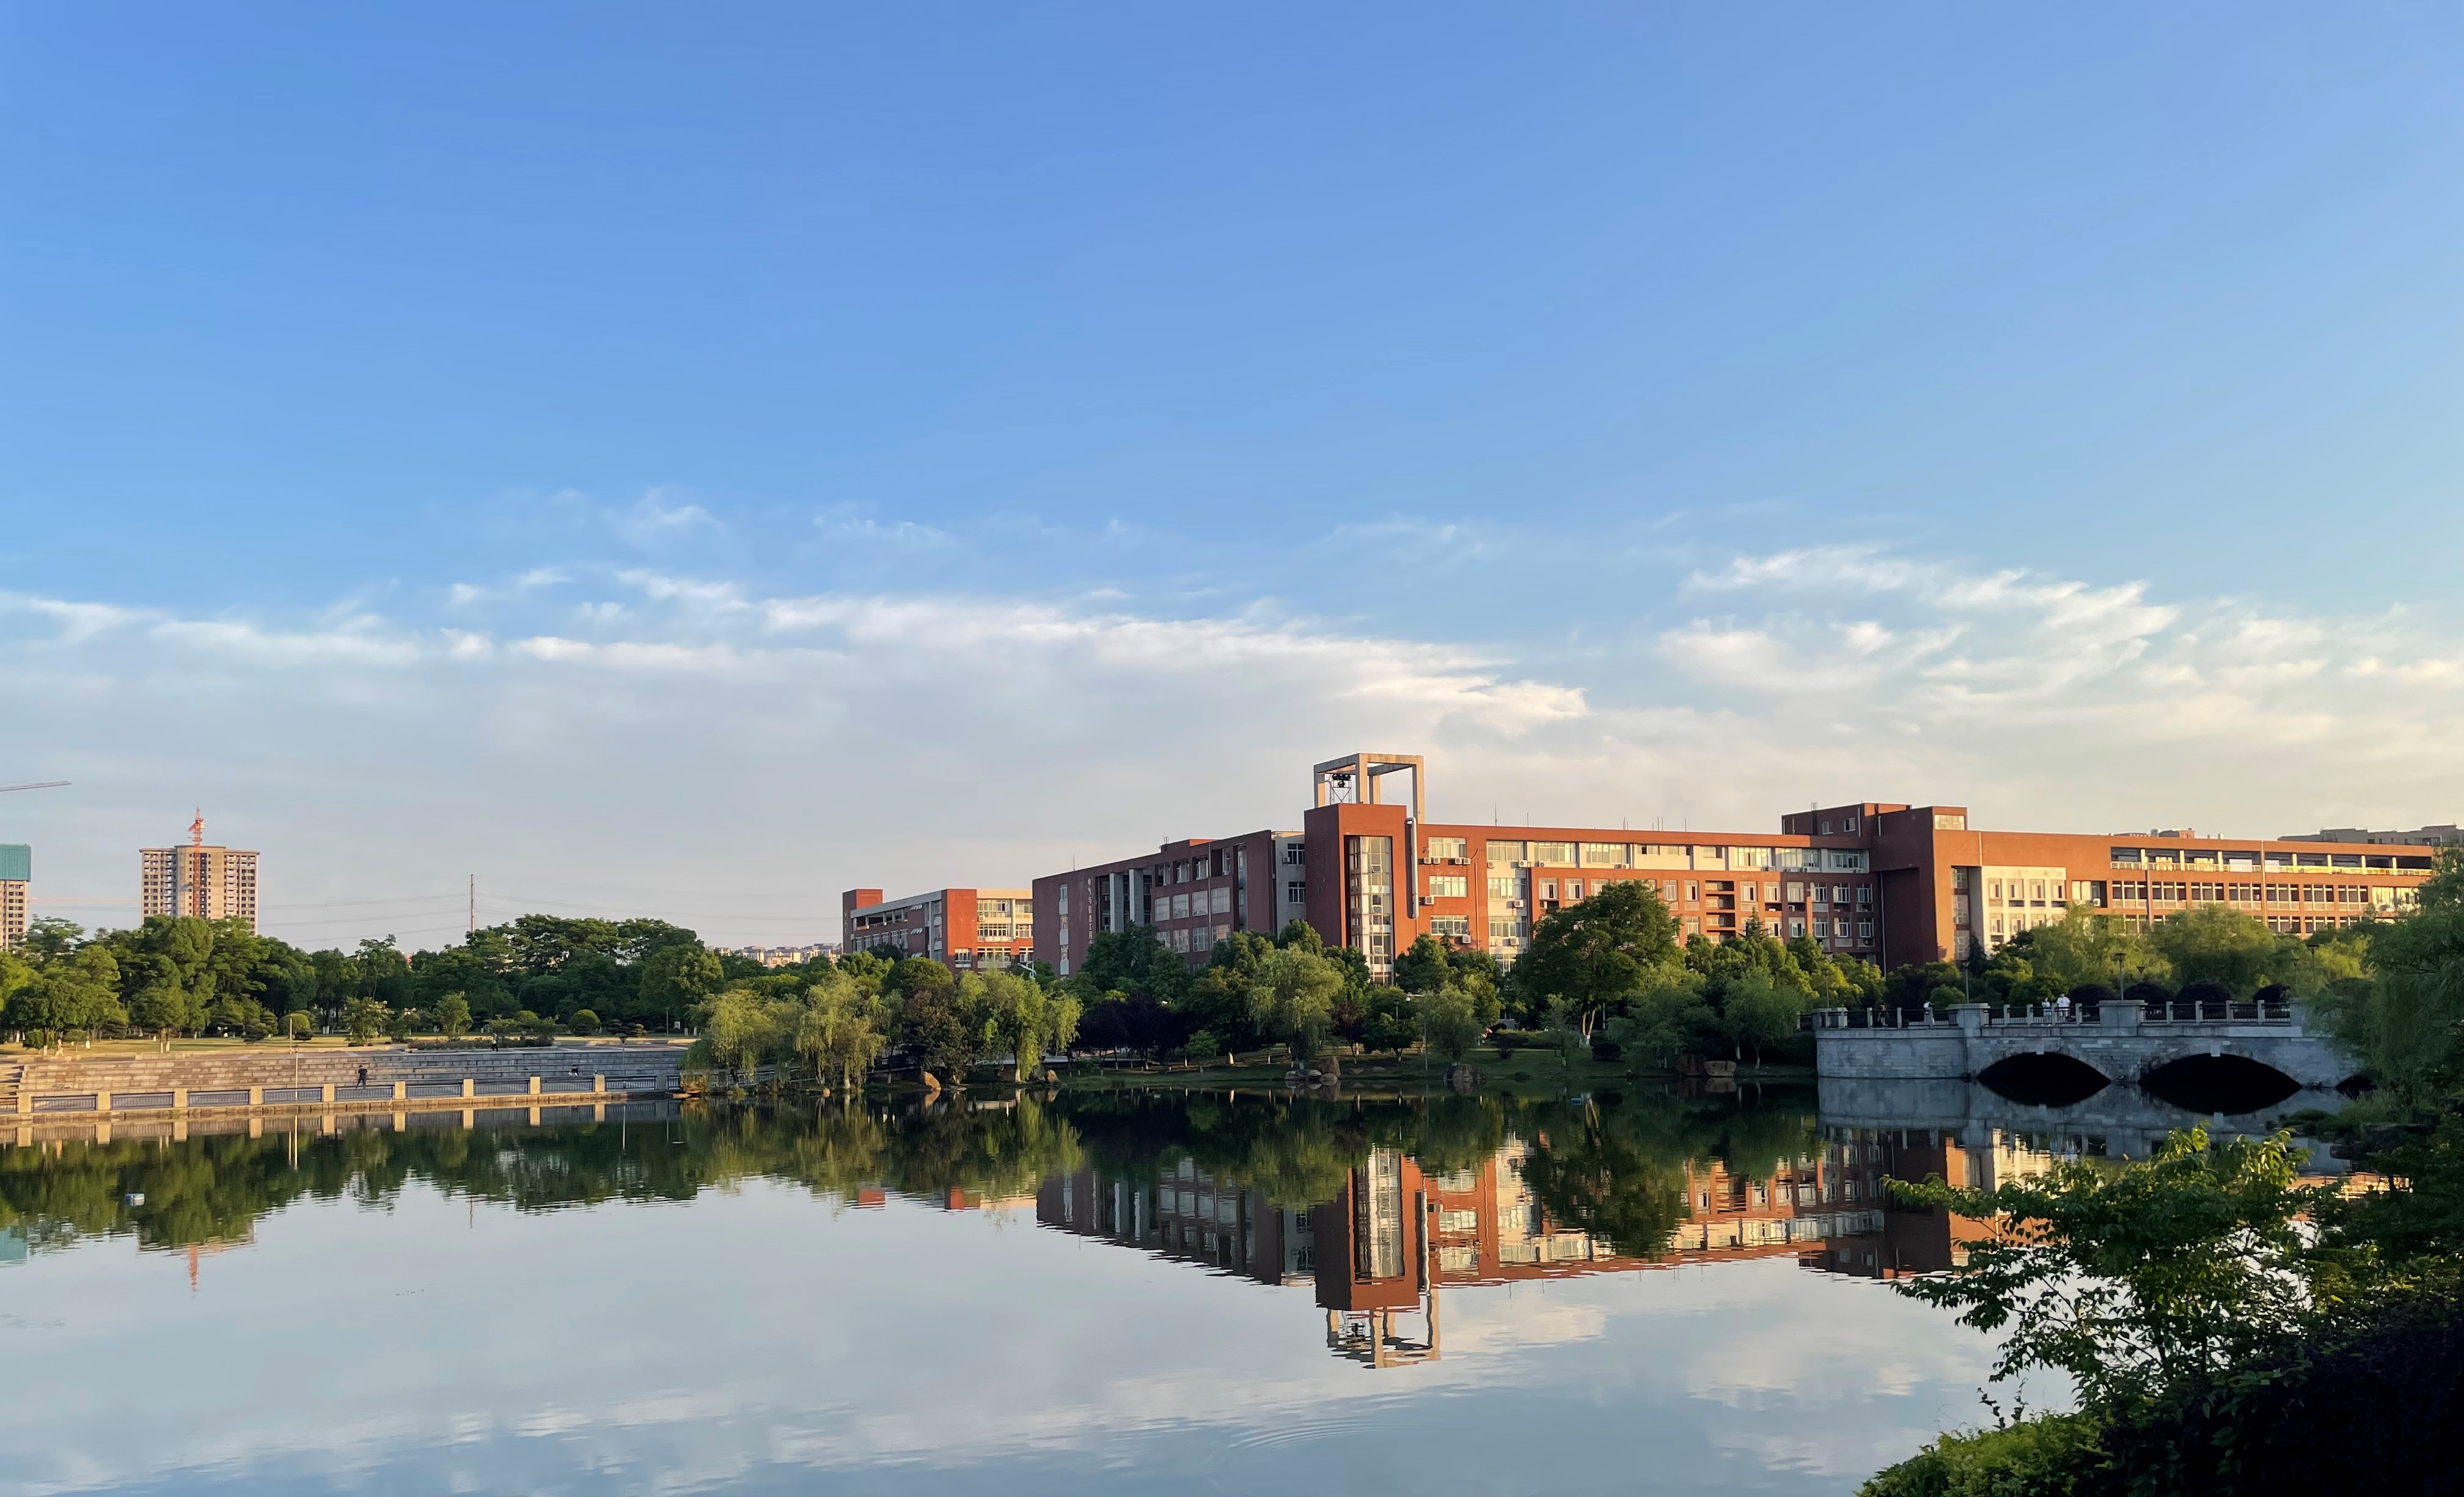
\includegraphics[width=0.8\linewidth]{img/fig1.jpg}
    \caption{一张示例图片}
    \label{fig:figure3}
\end{figure}
    % ================================================================


    % ==========================  参考文献  ==========================
    \clearpage
    \sanhaolineskip
    \bibliography{reference}
    \bibliographystyle{unsrt}
    \addcontentsline{toc}{section}{参考文献}
    % ================================================================


    % ============================ 致谢  =============================
    \clearpage
    \sanhaolineskip
    \section*{致\quad\ 谢}
        \xiaosi \song 

中文小四号宋体,英文用小四号Times New  Roman,首行缩进二个字,1.5倍行距。中文小四号宋体,英文用小四号Times New  Roman,首行缩进二个字,1.5倍行距。中文小四号宋体,英文用小四号Times New  Roman,首行缩进二个字,1.5倍行距。中文小四号宋体,英文用小四号Times New  Roman,首行缩进二个字,1.5倍行距。中文小四号宋体,英文用小四号Times New  Roman,首行缩进二个字,1.5倍行距。
    \addcontentsline{toc}{section}{致谢}
     % ================================================================
     

    % ============================ 附录  =============================
    \clearpage
    \sanhaolineskip
    \section*{附\quad\ 录}
        
\lipsum[1-2]
\lstinputlisting[
    style       =   Python,
    caption     =   {\bf example.py},
    label       =   {example.py}
]{code/example.py}
    \addcontentsline{toc}{section}{附录}
    % ================================================================

    
\end{document}
